\chapter{Background}
\label{chap:background}
This chapter will give some background theory for sampling. It is used as a basis for the implementation. 


\section{Sampling Theory}


%\subsection{Channelizer}
% 6.1 Channelizer . J. Harris, "Multirate Signal Processing for Communication Systems", p.140

\subsection{Multirate Signals}
\label{sec:multirate}
In Digital Signal Processing there are systems that require different sampling rates from each other. A multirate filter seeks to make it possible to change the sampling rate to make it possible to use in the other system. 

\subsubsection{Decimation}
% use anti aliasing lowpass filter and then downsample
Decimation is the process of reducing the sample rate. The process is achieved by first remove unwanted high frequency components to negate aliasing, usually by a low pass filter. Afterwards a downsampler keeps every nth sample of the input signal and removes the rest.\cite{harris_multirate_2022} 

Relationship between the sample rates is:
\begin{equation}
    f_{s,reduced} = \frac{f_{s,original}}{M}
\end{equation}
\cite{lyons_understanding_2011}


\subsubsection{Interpolation}
% upsampler with an anti imaging lowpass filter
Assume a sampled signal $x[n]$ with $n$ samples. The goal of the interpolation is to increase the sampling rate of sampled signal. In contrast with decimation, interpolation needs to calculate additional sampled values. The signal is usually upsampled first with zeros and then filtered using a low pass filter.


% example with linear interpolation with figure

Upsampling is ...
\cite{harris_multirate_2022}

\subsection{Lagrange Interpolation}
Lagrange interpolation utilizes polynomials to calculate the interpolated value.  Given a set of n distinct points $(x_0, y_0), (x_1, y_1), ..., (x_n, y_n)$. Lagrange theorem states that there exist a unique polynomial $P(x)$ of degree at most $n$ that passes through all these points. The Lagrange interpolation polynomial $L(x)$ is given by:
\begin{equation}
    P(x) = \sum_{i=0}^{n} y_i * L_i(x)
\end{equation}

$L_i(x)$ is the Lagrange basis polynomials defined as:

\begin{equation}
    L_i(x) = \prod_{_{\substack{j=0 \\ j\neq i}}}^n \frac{x - x_j}{x_i - x_j}
\end{equation} 
\cite{kreyszig_advanced_2011}

% include figure
% https://encyclopediaofmath.org/wiki/Lagrange_interpolation_formula?
% https://www.dsprelated.com/blogimages/JosefHoffmann/Farrow_Filter.pdf
\subsection{Sample Rate Conversion}


\subsection{Polyphase structure}

\section{\acrfull{asrc}}
% how the classical approach to arbitrary sample rate conversion is
% Upsample then downsample
The ratio in which the sample rate of a signal is resampled is often denoted as a fraction $P/Q$, where $P$ and $Q$ are integers \cite{harris_multirate_2022}
. This representation allows for both rational and irrational conversion ratios, though the latter requires approximation.

Consider a discrete-time signal $x[n]$ obtained by sampling a continuous-time signal $x(t)$ at a rate $fs$. The process of arbitrary sample rate conversion involves reconstructing $x(t)$ and resampling it at a new rate $fs'$.

\subsection{Rational}
A rational sample rate conversion occurs when the ratio $P/Q$ can be expressed exactly as a fraction of two integers. For example, having a ratio of $5/3$, it would be as simply as first oversampling by 5 and then downsample with 3. This can be done with a simple polyphase filter structure. 
% add figure

\subsection{Irrational}
To represent irrational numbers with high accuracy, it's frequently necessary to use large values for both $P$ and $Q$. However, this can lead to practical implementation issues due to the computational complexity of high order filters. These high order filters also causes resource constraints due to the requirements of large memories for the coefficients \cite{ramstad_digital_1984}. Multiple techniques have been used to address this problem.

\subsection{Variable fractional delay}
Variable fractional delay is one solution to \acrshort{asrc}. By introducing a time delay $D$, one can derive a new sample period $T'$ that allows for precise resampling between arbitrary input and output rates. This concept can be formalized as:
\begin{equation}
    T' = T + D
\end{equation}
Where $T$ is the input sample period and $D$ is the fractional delay. This new sample period $T'$ makes it possible to generate output samples at the desired sample rate. The fractional delay $D$ is typically a time-varying parameter that changes for each output sample. It can be expressed as:
\begin{equation}
    D(m) = mT' - nT
\end{equation}
Where $m$ is the output sample index, while $n$ is the input sample index.

% formulas to explain variable fractional delay


\subsection{Farrow filter}
One implementation of variable fractional delay is the farrow filter \cite{farrow_continuously_1988}. The farrow utilizes polynomials for the filters impulse response. 

% https://en.wikipedia.org/wiki/Horner%27s_method
% The polynomial is generally evaluated using the Horner scheme

%\section{Digital Filtering}
% https://en.wikipedia.org/wiki/Parks%E2%80%93McClellan_filter_design_algorithm
%\subsection{FIR Filter}

\section{\acrfull{fpga}}
% short intro to what fpgas are
\acrshort{fpga}s are integrated circuits that can be reconfigured by users to implement custom digital designs. Unlike fixed-function chips, FPGAs offer flexibility through an array of programmable logic elements (LEs) or configurable logic blocks (CLBs).

% how they work



% maybe a figure?

% applications


% 
% https://www.xilinx.com/products/silicon-devices/fpga/what-is-an-fpga.html
% 

\subsection{\acrshort{amba} \acrshort{axi}}
The \acrfull{axi} is part of ARM's \acrfull{amba} family of on-chip interconnect specifications. The \acrshort{axi} interconnect allows for different types of communications between IP blocks in a system-on-chip design. \acrshort{axi}4 is the newest version released in 2010 a part of the \acrshort{amba} 4.0.

\noindent There are three main types of \acrshort{axi} interfaces:
% https://docs.amd.com/v/u/en-US/ug761_axi_reference_guide
\begin{itemize}
    \item \textbf{AXI4:} Designed for high-performance memory-mapped operations. 
    \item \textbf{AXI4-Lite:} Suitable for simple, low-bandwidth memory-mapped communcation.
    \item \textbf{AXI4-Stream:} Optimized for high-speed streaming data transfer.
\end{itemize}

\acrshort{axi} works as a master-slave protocol. The master device initiate transactions by a request, and the slave device responds to the request by either writing or reading data. These transactions is accomplished by utilizing five independent channels: 
\begin{itemize}
    \item Write request
    \item Write data
    \item Write response
    \item Read request
    \item Read data
\end{itemize}
% file:///home/jacobk/Downloads/IHI0022K_amba_axi_protocol_spec.pdf
This channel architecture allows for efficient data transfer and enables advanced features such as out-of-order transaction completion and simultaneous read and write operations. The independence of these channels also provides flexibility in system design, allowing for optimized data flow and improved overall system performance. Additionally, this structure supports burst transfers, where multiple data items can be transferred in a single transaction. \cref{fig:axi_transaction} shows an transaction of a read request, illustrating how these channels interact during a typical AXI operation.

\begin{figure}[h]
    \centering
    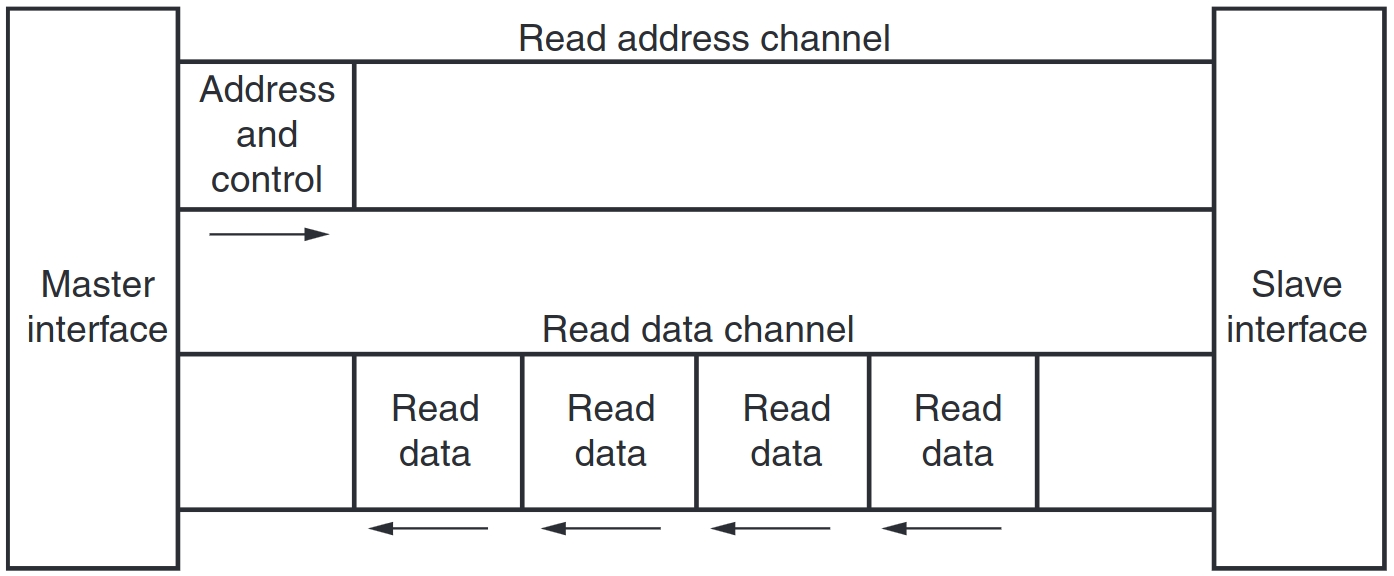
\includegraphics[width=0.9\textwidth]{figures/axi_transaction.jpeg}
    \caption{Transaction of read request}
    \label{fig:axi_transaction}
\end{figure}



\subsubsection{\acrshort{axi}-Stream}
% write about axi stream


% include figure of bits of data

\acrshort{axi}-Stream is used in the hardware implementation.


\subsection{Resource Utilization}
\subsubsection{LUTs}
\subsubsection{Memory blocks}
\subsubsection{\acrshort{mac}}
\acrfull{mac}


\subsection{Fixed-Point Arithmetic}
\section{Performance Metrics}
\subsection{Efficiency}
\subsection{Error}
\subsection{Computational Complexity}